% Options for packages loaded elsewhere
\PassOptionsToPackage{unicode}{hyperref}
\PassOptionsToPackage{hyphens}{url}
%
\documentclass[
  man]{apa6}
\usepackage{amsmath,amssymb}
\usepackage{iftex}
\ifPDFTeX
  \usepackage[T1]{fontenc}
  \usepackage[utf8]{inputenc}
  \usepackage{textcomp} % provide euro and other symbols
\else % if luatex or xetex
  \usepackage{unicode-math} % this also loads fontspec
  \defaultfontfeatures{Scale=MatchLowercase}
  \defaultfontfeatures[\rmfamily]{Ligatures=TeX,Scale=1}
\fi
\usepackage{lmodern}
\ifPDFTeX\else
  % xetex/luatex font selection
\fi
% Use upquote if available, for straight quotes in verbatim environments
\IfFileExists{upquote.sty}{\usepackage{upquote}}{}
\IfFileExists{microtype.sty}{% use microtype if available
  \usepackage[]{microtype}
  \UseMicrotypeSet[protrusion]{basicmath} % disable protrusion for tt fonts
}{}
\makeatletter
\@ifundefined{KOMAClassName}{% if non-KOMA class
  \IfFileExists{parskip.sty}{%
    \usepackage{parskip}
  }{% else
    \setlength{\parindent}{0pt}
    \setlength{\parskip}{6pt plus 2pt minus 1pt}}
}{% if KOMA class
  \KOMAoptions{parskip=half}}
\makeatother
\usepackage{xcolor}
\usepackage{graphicx}
\makeatletter
\def\maxwidth{\ifdim\Gin@nat@width>\linewidth\linewidth\else\Gin@nat@width\fi}
\def\maxheight{\ifdim\Gin@nat@height>\textheight\textheight\else\Gin@nat@height\fi}
\makeatother
% Scale images if necessary, so that they will not overflow the page
% margins by default, and it is still possible to overwrite the defaults
% using explicit options in \includegraphics[width, height, ...]{}
\setkeys{Gin}{width=\maxwidth,height=\maxheight,keepaspectratio}
% Set default figure placement to htbp
\makeatletter
\def\fps@figure{htbp}
\makeatother
\setlength{\emergencystretch}{3em} % prevent overfull lines
\providecommand{\tightlist}{%
  \setlength{\itemsep}{0pt}\setlength{\parskip}{0pt}}
\setcounter{secnumdepth}{-\maxdimen} % remove section numbering
% Make \paragraph and \subparagraph free-standing
\makeatletter
\ifx\paragraph\undefined\else
  \let\oldparagraph\paragraph
  \renewcommand{\paragraph}{
    \@ifstar
      \xxxParagraphStar
      \xxxParagraphNoStar
  }
  \newcommand{\xxxParagraphStar}[1]{\oldparagraph*{#1}\mbox{}}
  \newcommand{\xxxParagraphNoStar}[1]{\oldparagraph{#1}\mbox{}}
\fi
\ifx\subparagraph\undefined\else
  \let\oldsubparagraph\subparagraph
  \renewcommand{\subparagraph}{
    \@ifstar
      \xxxSubParagraphStar
      \xxxSubParagraphNoStar
  }
  \newcommand{\xxxSubParagraphStar}[1]{\oldsubparagraph*{#1}\mbox{}}
  \newcommand{\xxxSubParagraphNoStar}[1]{\oldsubparagraph{#1}\mbox{}}
\fi
\makeatother
% definitions for citeproc citations
\NewDocumentCommand\citeproctext{}{}
\NewDocumentCommand\citeproc{mm}{%
  \begingroup\def\citeproctext{#2}\cite{#1}\endgroup}
\makeatletter
 % allow citations to break across lines
 \let\@cite@ofmt\@firstofone
 % avoid brackets around text for \cite:
 \def\@biblabel#1{}
 \def\@cite#1#2{{#1\if@tempswa , #2\fi}}
\makeatother
\newlength{\cslhangindent}
\setlength{\cslhangindent}{1.5em}
\newlength{\csllabelwidth}
\setlength{\csllabelwidth}{3em}
\newenvironment{CSLReferences}[2] % #1 hanging-indent, #2 entry-spacing
 {\begin{list}{}{%
  \setlength{\itemindent}{0pt}
  \setlength{\leftmargin}{0pt}
  \setlength{\parsep}{0pt}
  % turn on hanging indent if param 1 is 1
  \ifodd #1
   \setlength{\leftmargin}{\cslhangindent}
   \setlength{\itemindent}{-1\cslhangindent}
  \fi
  % set entry spacing
  \setlength{\itemsep}{#2\baselineskip}}}
 {\end{list}}
\usepackage{calc}
\newcommand{\CSLBlock}[1]{\hfill\break\parbox[t]{\linewidth}{\strut\ignorespaces#1\strut}}
\newcommand{\CSLLeftMargin}[1]{\parbox[t]{\csllabelwidth}{\strut#1\strut}}
\newcommand{\CSLRightInline}[1]{\parbox[t]{\linewidth - \csllabelwidth}{\strut#1\strut}}
\newcommand{\CSLIndent}[1]{\hspace{\cslhangindent}#1}
\ifLuaTeX
\usepackage[bidi=basic]{babel}
\else
\usepackage[bidi=default]{babel}
\fi
\babelprovide[main,import]{english}
% get rid of language-specific shorthands (see #6817):
\let\LanguageShortHands\languageshorthands
\def\languageshorthands#1{}
% Manuscript styling
\usepackage{upgreek}
\captionsetup{font=singlespacing,justification=justified}

% Table formatting
\usepackage{longtable}
\usepackage{lscape}
% \usepackage[counterclockwise]{rotating}   % Landscape page setup for large tables
\usepackage{multirow}		% Table styling
\usepackage{tabularx}		% Control Column width
\usepackage[flushleft]{threeparttable}	% Allows for three part tables with a specified notes section
\usepackage{threeparttablex}            % Lets threeparttable work with longtable

% Create new environments so endfloat can handle them
% \newenvironment{ltable}
%   {\begin{landscape}\centering\begin{threeparttable}}
%   {\end{threeparttable}\end{landscape}}
\newenvironment{lltable}{\begin{landscape}\centering\begin{ThreePartTable}}{\end{ThreePartTable}\end{landscape}}

% Enables adjusting longtable caption width to table width
% Solution found at http://golatex.de/longtable-mit-caption-so-breit-wie-die-tabelle-t15767.html
\makeatletter
\newcommand\LastLTentrywidth{1em}
\newlength\longtablewidth
\setlength{\longtablewidth}{1in}
\newcommand{\getlongtablewidth}{\begingroup \ifcsname LT@\roman{LT@tables}\endcsname \global\longtablewidth=0pt \renewcommand{\LT@entry}[2]{\global\advance\longtablewidth by ##2\relax\gdef\LastLTentrywidth{##2}}\@nameuse{LT@\roman{LT@tables}} \fi \endgroup}

% \setlength{\parindent}{0.5in}
% \setlength{\parskip}{0pt plus 0pt minus 0pt}

% Overwrite redefinition of paragraph and subparagraph by the default LaTeX template
% See https://github.com/crsh/papaja/issues/292
\makeatletter
\renewcommand{\paragraph}{\@startsection{paragraph}{4}{\parindent}%
  {0\baselineskip \@plus 0.2ex \@minus 0.2ex}%
  {-1em}%
  {\normalfont\normalsize\bfseries\itshape\typesectitle}}

\renewcommand{\subparagraph}[1]{\@startsection{subparagraph}{5}{1em}%
  {0\baselineskip \@plus 0.2ex \@minus 0.2ex}%
  {-\z@\relax}%
  {\normalfont\normalsize\itshape\hspace{\parindent}{#1}\textit{\addperi}}{\relax}}
\makeatother

\makeatletter
\usepackage{etoolbox}
\patchcmd{\maketitle}
  {\section{\normalfont\normalsize\abstractname}}
  {\section*{\normalfont\normalsize\abstractname}}
  {}{\typeout{Failed to patch abstract.}}
\patchcmd{\maketitle}
  {\section{\protect\normalfont{\@title}}}
  {\section*{\protect\normalfont{\@title}}}
  {}{\typeout{Failed to patch title.}}
\makeatother

\usepackage{xpatch}
\makeatletter
\xapptocmd\appendix
  {\xapptocmd\section
    {\addcontentsline{toc}{section}{\appendixname\ifoneappendix\else~\theappendix\fi\\: #1}}
    {}{\InnerPatchFailed}%
  }
{}{\PatchFailed}
\keywords{keywords\newline\indent Word count: X}
\DeclareDelayedFloatFlavor{ThreePartTable}{table}
\DeclareDelayedFloatFlavor{lltable}{table}
\DeclareDelayedFloatFlavor*{longtable}{table}
\makeatletter
\renewcommand{\efloat@iwrite}[1]{\immediate\expandafter\protected@write\csname efloat@post#1\endcsname{}}
\makeatother
\usepackage{lineno}

\linenumbers
\usepackage{csquotes}
\ifLuaTeX
  \usepackage{selnolig}  % disable illegal ligatures
\fi
\usepackage{bookmark}
\IfFileExists{xurl.sty}{\usepackage{xurl}}{} % add URL line breaks if available
\urlstyle{same}
\hypersetup{
  pdftitle={The title},
  pdfauthor={First Author1 \& Ernst-August Doelle1,2},
  pdflang={en-EN},
  pdfkeywords={keywords},
  hidelinks,
  pdfcreator={LaTeX via pandoc}}

\title{The title}
\author{First Author\textsuperscript{1} \& Ernst-August Doelle\textsuperscript{1,2}}
\date{}


\shorttitle{Title}

\authornote{

Add complete departmental affiliations for each author here. Each new line herein must be indented, like this line.
Enter author note here.

The authors made the following contributions. First Author: Conceptualization, Writing - Original Draft Preparation, Writing - Review \& Editing; Ernst-August Doelle: Writing - Review \& Editing, Supervision.

Correspondence concerning this article should be addressed to First Author, Postal address. E-mail: \href{mailto:my@email.com}{\nolinkurl{my@email.com}}

}

\affiliation{\vspace{0.5cm}\textsuperscript{1} Wilhelm-Wundt-University\\\textsuperscript{2} Konstanz Business School}

\abstract{%
One or two sentences providing a \textbf{basic introduction} to the field, comprehensible to a scientist in any discipline.
Two to three sentences of \textbf{more detailed background}, comprehensible to scientists in related disciplines.
One sentence clearly stating the \textbf{general problem} being addressed by this particular study.
One sentence summarizing the main result (with the words ``\textbf{here we show}'' or their equivalent).
Two or three sentences explaining what the \textbf{main result} reveals in direct comparison to what was thought to be the case previously, or how the main result adds to previous knowledge.
One or two sentences to put the results into a more \textbf{general context}.
Two or three sentences to provide a \textbf{broader perspective}, readily comprehensible to a scientist in any discipline.
}



\begin{document}
\maketitle

Death is something each of us must learn to cope with, whether in
healthy ways or less so. These issues may be at front of mind for many
in light of the COVID-19 pandemic. Various existential philosophers and
psychologists have proposed ways in which we deal with the awareness of
death and the anxiety this awareness often causes. Psychoanalyst Erik
Erikson (1950) proposed that during mid-life one becomes
acutely aware of their oncoming death and is motivated to care for
things which will outlast themselves. He called this act of caring
generativity. In \emph{The Denial of Death}, philosopher Ernest Becker
(\textbf{becker1973?}) posits that humans undertake immortality projects to curb
their sense of vulnerability to death. Similarly, psychiatrist Robert
Jay Lifton (\textbf{lifton1979?}), a mentee of Erikson, described the awareness
of death as being ever present and motivating us to create symbols,
thereby allowing us to imagine ourselves as symbolically immortalized.
Existential psychiatrist Irvin Yalom (\textbf{yalom2008?}) notes that many of
his clients experiencing anxiety about their death take comfort in
``rippling,'' the idea that one's lasting effects on the world will ripple
out and influence the world after they have died.

Although these thinkers use different terminology, there are several
common themes among their ideas. (1) Our physical death is an
inevitability, and we often find our awareness of its inevitability to
be aversive. This aversion may be referred to variously as angst,
death-anxiety, despair, being-towards-death, terror, and so on. However,
(2) we take comfort in the idea that other, non-physical parts of us
continue to exist indefinitely after our biological death, through
mechanisms such as the heroic archetype and symbolic self. (3) Finally,
we can take action to promote these non-physical aspects of the self,
such as through search for meaning, sense of immortality, care,
generativity, and rippling.

One of these bodies of thought, called symbolic immortality, was
originally theorized by Lifton (\textbf{lifton1979?}), who thought that
awareness of death drives a fundamental human desire for a sense of
continuity lasting beyond the lifespan. Essentially, humans are
meaning-seeking creatures, and throughout our lives, this search for
meaning involves an evolving psychological imagery of life and death.
Death, or the transient nature of life, threatens our search for
meaning. Lifton thought that if we could achieve what we believe to be
some form of immortality, we could overcome this loss of meaning, and
the awareness of death could instead drive an inner vitality (imagery
associated with connection, integrity, and movement). If this drive
toward vitality is lost, we are vulnerable to a psychic numbness or
death-in-life (imagery associated with separation, disintegration, and
stasis). In Lifton's own words, ``Death does indeed bring about
biological and psychic annihilation. But life includes symbolic
perceptions of connections that precede and outlast that annihilation''
(\textbf{lifton1979?}).

Lifton (\textbf{lifton1979?}) proposed five modes of experience or ways of
achieving symbolic immortality: The biological (or biosocial) mode in
which one lives on through their genetic and sociocultural progeny, the
creative mode in which one's accomplishments and contribution outlast
oneself, the natural mode in which one feels they are a part of the
broader universe, the spiritual mode in which one seeks to transcend the
physical realm to a higher spiritual realm beyond death, and the mode of
experiential transcendence in which one experiences a phenomenological
state of flow. The experiential mode must occur in the context of at
least one of the other four to really be considered transcendent, but it
is thought to have a great capacity to bring about personal change.

Claims of how we suppress death-anxiety have been investigated
experimentally, primarily through the paradigm of Terror Management
Theory (TMT). Based on the theories of Ernest Becker, TMT posits that
human awareness of death is always present to some degree. This
awareness of our inevitable death, coupled with a strong aversion to
thoughts of death, causes terror and is pushed out of our consciousness
by our creation of meaning systems (Greenberg, Pyszczynski, \& Solomon, 1986). TMT proposes that
self-esteem, interpersonal relationships, and cultural worldview work
together to buffer against our anxiety about death. It is assumed that
these buffers suppress thoughts of death by providing a sense of
symbolic immortality, though little systematic research has been
conducted on this construct. The results of this buffering process are
not always positive. For example, experimentally priming mortality
salience can lead to more positive attitudes toward in-group members but
harsher negative attitudes toward out-group members (Greenberg et al., 1990).

TMT refers to a person's awareness of death as mortality salience (MS).
The MS hypothesis of TMT posits than an increase in one's awareness of
death causes an increase in compensatory behaviors to lower their death
anxiety, either by distracting from the awareness of death or by the
promotion of meaningful cultural worldviews. In the MS paradigm,
experimentally priming a participant's awareness of death (for example,
by having participants write about death and then complete a distraction
task) is thought to cause an increase in compensatory buffers. A
meta-analysis of 277 experiments found mortality salience to have a
robust, moderate overall effect size: \emph{r}(276) = 0.35, \emph{p} = .00
(Burke, Martens, \& Faucher, 2010). Altogether, these experiments provide convincing evidence
for TMT and the MS hypothesis in particular.

Though some avoidance of (or buffering against) death anxiety is thought
to be universal and has the potential to increase interpersonal
conflict, awareness of death through symbolic immortality may also have
potential as a positive force. In particular, it is thought to be an
underlying motive for what Erikson referred to as generativity.
Generativity is the seventh of eight proposed stages in Erikson's
(1950) theory of psychosocial development, which he associated
with midlife and described as ``the concern in establishing and guiding
the next generation'' (E. H. Erikson, 1963, p. 267). Little systematic research
was conducted on this subject until the 1980's. Kotre (1984)
expanded on the theory and proposed that the drive for generativity was
related to a motive to expand the sense of self beyond the lifetime,
especially in light of the fear of death.

McAdams and de St.~Aubin (1992) sought to formalize the study
of generativity as a multidimensional construct. Their seven components
of generativity include cultural demand, inner desire (for symbolic
immortality and community), concern (for the next generation), belief
(in the human species), commitment, action, and narration (of
generativity within one's life story). In addition to a quantitative
measure of generative concern (the Loyola Generativity Scale), they
developed a system for content analysis of autobiographical episodes
pertaining to generativity, and symbolic immortality is one of the five
themes they found. Here they define symbolic immortality as ``any
reference to leaving a legacy, having an enduring influence, or leaving
behind products that will outlive one's physical existence,'' a theme
clearly related to both Lifton's and Erikson's theories (McAdams \& St. Aubin, 1992, p. 1011).

These research areas depend on the construct of symbolic immortality for
their theoretical frameworks, but few researchers have attempted to
systematically and quantitatively assess this construct. Two attempts
have been made to develop such a measurement: Drolet's (1990)
Sense of Symbolic Immortality Scale and Mathews and Kling's
(1988) measure of symbolic immortality, based on an original
questionnaire by Mathews and Mister (1987).

Drolet (1990) developed the Sense of Symbolic Immortality Scale
based on Robert J. Lifton's theory of symbolic immortality and its five
modes of experience. Drolet studied 136 adults, ages 18-30 and 30-40,
and hypothesized that those in their 30's (established adults) would
have a greater sense of symbolic immortality than the young adults
(18-30). The measure is inherently subjective, not only by the nature of
self-report, but in that the scale seeks to measure what a person
\emph{believes} and how they \emph{feel} about these subjects. The scale as a
whole had a high internal consistency (\(\alpha\) = .91) and test-retest
reliability was \emph{r} = .97. Internal consistency of subscales for the
five theoretical modes of immortality was mixed. Of the five, spiritual
immortality was the most distinct from the scale as a whole and the
other subscales. Factor analysis showed three factors, mapping onto
biosocial, creative, and spiritual. The transcendent and natural items
may be closely related to biosocial.

Moving beyond the scale development itself, SSI correlated negatively
with Templer's Death Anxiety Scale and had a strong (\emph{r} = .84) positive
relationship with Maholick's Purpose in Life Test (Drolet, 1990). In
interpreting the very strong correlation, the author suggests that SSI
is a broader construct than Purpose in Life and the scale itself may be
less prone to social desirability effects than the PIL, although this
had not been directly tested. Age group was also related, with
established adults having a higher SSI, particularly in the biosocial
and creative domains.

We see multiple issues with using the Symbolic Immortality Scale. First,
the study was underpowered, conducting exploratory factor analysis of 67
items using a sample of 136. Second, the scale was developed in French,
and we do not take for granted the psychometric properties of a
translated version. Third and most fundamentally, the scale has poor
face validity and appears to measure the constructs theorized to
symbolically immortalize rather than a sense of symbolic immortality
directly. For example, the scale includes items such as ``My sex life
contributes greatly to my well-being'', ``Intimate relationships scare
me'', and ``I am sure of who I am.'' Although related to the constructs
(such as interpersonal relationships and self-esteem) which
theoretically help cope with death, it is unclear how these items
represent the construct of symbolic immortality itself.

Mathews and Mister (1987) also developed a scale pertaining to
symbolic immortality, sensation seeking, and psychic numbness in a study
including 400 adults. Experiential transcendence was operationalized as
similar to Zuckerman's (1979) sensation seeking, which may
not fully capture the original intent (the experience of losing
oneself). Items were mapped onto five factors, and the five factors
largely aligned with Lifton's constructs. Although internal consistency
was at least acceptable for each factor, goodness of fit statistics are
not reported. Some studies have used a revised version of the scale by
Mathews and Kling (1988), who adapted it for a study on
prosocial behavior in the context of nonprofit volunteer motivation.
They reported similar results for their revised scale. The items on
these scales seem to have more face validity than the scale by Drolet,
but some factors seem more behavioral and unnecessarily specific:
pertaining to one's religiosity or biological children, whereas Lifton's
theory allows for a broader interpretation of these dimensions. The
Nature and Creative factors seem most useful and theoretically aligned
with Lifton.

Much more advanced factor analysis methods have been developed since the
1980s, but to our knowledge, these scales have not been tested with more
robust tools. The goal of the present research is to develop an
up-to-date symbolic immortality scale that more directly measures one's
sense of symbolic immortality and which contains items more generally
applicable to broad groups of participants (e.g., regardless of a
person's religious beliefs and parental status). We have attempted to
use current best practices for scale development and analysis.

\section{Method}\label{method}

\subsection{Participants}\label{participants}

\subsection{Material}\label{material}

\subsection{Procedure}\label{procedure}

\subsection{Data analysis}\label{data-analysis}

\section{Results}\label{results}

\subsection{Data Screening}\label{data-screening}

\begin{verbatim}
## [1] 352
\end{verbatim}

\begin{verbatim}
## [1] 353
\end{verbatim}

\begin{verbatim}
## [1] 326
\end{verbatim}

\begin{verbatim}
## [1] 326
\end{verbatim}

\subsection{EFA}\label{efa}

\subsubsection{Number of Factors}\label{number-of-factors}

also do five

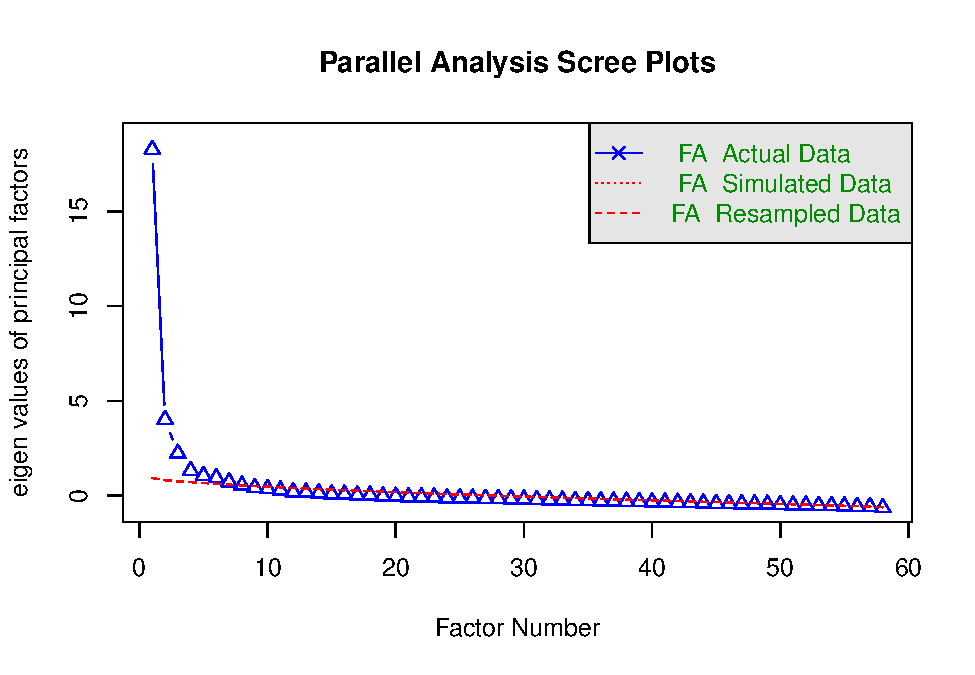
\includegraphics{manuscript_files/figure-latex/unnamed-chunk-1-1.pdf}

\begin{verbatim}
## Parallel analysis suggests that the number of factors =  7  and the number of components =  NA
\end{verbatim}

\begin{verbatim}
## [1] 5
\end{verbatim}

\begin{verbatim}
## [1] 7
\end{verbatim}

\subsubsection{Simple Structure}\label{simple-structure}

\begin{verbatim}
## Factor Analysis using method =  ml
## Call: fa(r = efaDF, nfactors = 2, rotate = "oblimin", fm = "ml")
## Standardized loadings (pattern matrix) based upon correlation matrix
##         ML1   ML2    h2   u2 com
## Q2_1   0.57  0.15 0.436 0.56 1.1
## Q2_2   0.77 -0.05 0.552 0.45 1.0
## Q2_3   0.76 -0.08 0.528 0.47 1.0
## Q2_4   0.70  0.05 0.523 0.48 1.0
## Q2_5   0.73 -0.10 0.466 0.53 1.0
## Q2_6   0.72  0.06 0.561 0.44 1.0
## Q2_7   0.47  0.07 0.259 0.74 1.0
## Q2_8   0.65 -0.03 0.408 0.59 1.0
## Q2_9   0.63  0.01 0.405 0.60 1.0
## Q2_10  0.58 -0.05 0.308 0.69 1.0
## Q2_11  0.18  0.64 0.546 0.45 1.2
## Q2_12 -0.05  0.92 0.805 0.19 1.0
## Q2_13  0.11  0.18 0.066 0.93 1.6
## Q2_14  0.66  0.06 0.480 0.52 1.0
## Q2_15  0.68 -0.08 0.421 0.58 1.0
## Q2_16  0.79 -0.08 0.571 0.43 1.0
## Q2_17 -0.01  0.92 0.836 0.16 1.0
## Q2_18  0.14  0.75 0.686 0.31 1.1
## Q2_19  0.46  0.12 0.286 0.71 1.1
## Q2_20  0.64 -0.11 0.354 0.65 1.1
## Q4_1   0.71 -0.06 0.468 0.53 1.0
## Q4_2   0.60 -0.05 0.328 0.67 1.0
## Q4_3   0.60 -0.06 0.335 0.66 1.0
## Q4_4   0.52  0.13 0.351 0.65 1.1
## Q4_5   0.67 -0.06 0.410 0.59 1.0
## Q4_6   0.52  0.19 0.411 0.59 1.3
## Q4_7   0.31 -0.13 0.073 0.93 1.3
## Q4_8   0.34  0.07 0.148 0.85 1.1
## Q4_9   0.65  0.15 0.533 0.47 1.1
## Q4_10  0.68  0.03 0.481 0.52 1.0
## Q4_11  0.09  0.14 0.042 0.96 1.7
## Q4_12  0.40 -0.04 0.146 0.85 1.0
## Q4_13  0.23  0.38 0.286 0.71 1.7
## Q4_14  0.17  0.46 0.317 0.68 1.3
## Q4_15  0.63  0.04 0.421 0.58 1.0
## Q4_16  0.55  0.01 0.312 0.69 1.0
## Q4_17  0.12  0.51 0.336 0.66 1.1
## Q4_18  0.10  0.19 0.064 0.94 1.5
## Q4_19 -0.07  0.95 0.834 0.17 1.0
## Q5_1   0.07  0.78 0.670 0.33 1.0
## Q5_2   0.02  0.85 0.740 0.26 1.0
## Q5_3   0.09  0.50 0.305 0.70 1.1
## Q5_4   0.51  0.25 0.446 0.55 1.5
## Q5_5   0.14  0.00 0.021 0.98 1.0
## Q5_6   0.44  0.16 0.290 0.71 1.3
## Q5_7   0.59 -0.01 0.338 0.66 1.0
## Q5_8   0.68  0.04 0.491 0.51 1.0
## Q5_9   0.75 -0.03 0.547 0.45 1.0
## Q5_10 -0.06  0.85 0.669 0.33 1.0
## Q5_11 -0.02  0.15 0.020 0.98 1.0
## Q5_12  0.05  0.30 0.107 0.89 1.1
## Q5_13  0.74  0.04 0.574 0.43 1.0
## Q5_14  0.31 -0.04 0.085 0.91 1.0
## Q5_15  0.57  0.09 0.387 0.61 1.1
## Q5_17  0.49  0.15 0.334 0.67 1.2
## Q5_18  0.35  0.20 0.232 0.77 1.6
## Q5_19  0.52  0.25 0.466 0.53 1.4
## Q5_20  0.19 -0.06 0.029 0.97 1.2
## 
##                         ML1  ML2
## SS loadings           14.91 7.63
## Proportion Var         0.26 0.13
## Cumulative Var         0.26 0.39
## Proportion Explained   0.66 0.34
## Cumulative Proportion  0.66 1.00
## 
##  With factor correlations of 
##      ML1  ML2
## ML1 1.00 0.49
## ML2 0.49 1.00
## 
## Mean item complexity =  1.1
## Test of the hypothesis that 2 factors are sufficient.
## 
## df null model =  1653  with the objective function =  38.9 with Chi Square =  12870.73
## df of  the model are 1538  and the objective function was  12.63 
## 
## The root mean square of the residuals (RMSR) is  0.07 
## The df corrected root mean square of the residuals is  0.07 
## 
## The harmonic n.obs is  352 with the empirical chi square  5082.08  with prob <  0 
## The total n.obs was  352  with Likelihood Chi Square =  4161.82  with prob <  4.3e-240 
## 
## Tucker Lewis Index of factoring reliability =  0.747
## RMSEA index =  0.07  and the 90 % confidence intervals are  0.067 0.072
## BIC =  -4856.44
## Fit based upon off diagonal values = 0.96
## Measures of factor score adequacy             
##                                                    ML1  ML2
## Correlation of (regression) scores with factors   0.98 0.98
## Multiple R square of scores with factors          0.96 0.96
## Minimum correlation of possible factor scores     0.93 0.93
\end{verbatim}

\begin{verbatim}
## Factor Analysis using method =  ml
## Call: fa(r = efaDF %>% select(efa_loadings %>% filter(keep == "yes") %>% 
##     pull(question)), nfactors = 2, rotate = "oblimin", fm = "ml")
## Standardized loadings (pattern matrix) based upon correlation matrix
##         ML1   ML2    h2   u2 com
## Q2_1   0.57  0.15 0.435 0.56 1.1
## Q2_2   0.77 -0.06 0.551 0.45 1.0
## Q2_3   0.76 -0.08 0.529 0.47 1.0
## Q2_4   0.69  0.06 0.525 0.47 1.0
## Q2_5   0.73 -0.10 0.467 0.53 1.0
## Q2_6   0.72  0.06 0.561 0.44 1.0
## Q2_7   0.47  0.07 0.260 0.74 1.0
## Q2_8   0.65 -0.02 0.408 0.59 1.0
## Q2_9   0.63  0.01 0.406 0.59 1.0
## Q2_10  0.58 -0.05 0.306 0.69 1.0
## Q2_11  0.18  0.64 0.545 0.45 1.2
## Q2_12 -0.05  0.92 0.805 0.20 1.0
## Q2_14  0.66  0.05 0.477 0.52 1.0
## Q2_15  0.68 -0.08 0.422 0.58 1.0
## Q2_16  0.79 -0.08 0.572 0.43 1.0
## Q2_17 -0.01  0.92 0.837 0.16 1.0
## Q2_18  0.14  0.75 0.686 0.31 1.1
## Q2_19  0.46  0.13 0.287 0.71 1.1
## Q2_20  0.64 -0.10 0.353 0.65 1.0
## Q4_1   0.71 -0.06 0.469 0.53 1.0
## Q4_2   0.60 -0.06 0.329 0.67 1.0
## Q4_3   0.60 -0.05 0.335 0.67 1.0
## Q4_4   0.52  0.13 0.349 0.65 1.1
## Q4_5   0.67 -0.06 0.410 0.59 1.0
## Q4_6   0.52  0.20 0.413 0.59 1.3
## Q4_7   0.31 -0.13 0.072 0.93 1.4
## Q4_8   0.34  0.07 0.146 0.85 1.1
## Q4_9   0.65  0.14 0.533 0.47 1.1
## Q4_10  0.68  0.02 0.481 0.52 1.0
## Q4_12  0.40 -0.04 0.145 0.86 1.0
## Q4_13  0.23  0.38 0.285 0.72 1.7
## Q4_14  0.16  0.47 0.321 0.68 1.2
## Q4_15  0.63  0.04 0.423 0.58 1.0
## Q4_16  0.55  0.01 0.309 0.69 1.0
## Q4_17  0.12  0.51 0.329 0.67 1.1
## Q4_19 -0.07  0.95 0.835 0.16 1.0
## Q5_1   0.07  0.78 0.672 0.33 1.0
## Q5_2   0.02  0.85 0.742 0.26 1.0
## Q5_3   0.08  0.51 0.306 0.69 1.1
## Q5_4   0.51  0.25 0.446 0.55 1.5
## Q5_6   0.44  0.16 0.288 0.71 1.2
## Q5_7   0.59 -0.02 0.337 0.66 1.0
## Q5_8   0.68  0.04 0.489 0.51 1.0
## Q5_9   0.75 -0.02 0.549 0.45 1.0
## Q5_10 -0.06  0.85 0.666 0.33 1.0
## Q5_13  0.74  0.04 0.574 0.43 1.0
## Q5_14  0.31 -0.04 0.085 0.91 1.0
## Q5_15  0.57  0.09 0.388 0.61 1.1
## Q5_17  0.49  0.15 0.334 0.67 1.2
## Q5_18  0.35  0.20 0.230 0.77 1.6
## Q5_19  0.52  0.25 0.466 0.53 1.4
## 
##                         ML1  ML2
## SS loadings           14.80 7.39
## Proportion Var         0.29 0.14
## Cumulative Var         0.29 0.44
## Proportion Explained   0.67 0.33
## Cumulative Proportion  0.67 1.00
## 
##  With factor correlations of 
##      ML1  ML2
## ML1 1.00 0.49
## ML2 0.49 1.00
## 
## Mean item complexity =  1.1
## Test of the hypothesis that 2 factors are sufficient.
## 
## df null model =  1275  with the objective function =  35.47 with Chi Square =  11817.61
## df of  the model are 1174  and the objective function was  9.54 
## 
## The root mean square of the residuals (RMSR) is  0.06 
## The df corrected root mean square of the residuals is  0.06 
## 
## The harmonic n.obs is  352 with the empirical chi square  2962.25  with prob <  4.6e-155 
## The total n.obs was  352  with Likelihood Chi Square =  3164.31  with prob <  3.7e-182 
## 
## Tucker Lewis Index of factoring reliability =  0.794
## RMSEA index =  0.069  and the 90 % confidence intervals are  0.067 0.072
## BIC =  -3719.59
## Fit based upon off diagonal values = 0.98
## Measures of factor score adequacy             
##                                                    ML1  ML2
## Correlation of (regression) scores with factors   0.98 0.98
## Multiple R square of scores with factors          0.96 0.96
## Minimum correlation of possible factor scores     0.93 0.93
\end{verbatim}

\begin{verbatim}
## Factor Analysis using method =  ml
## Call: fa(r = efaDF, nfactors = 3, rotate = "oblimin", fm = "ml")
## Standardized loadings (pattern matrix) based upon correlation matrix
##         ML1   ML2   ML3    h2   u2 com
## Q2_1   0.47  0.17  0.20 0.445 0.56 1.6
## Q2_2   0.63 -0.03  0.28 0.572 0.43 1.4
## Q2_3   0.72 -0.05  0.08 0.528 0.47 1.0
## Q2_4   0.71  0.09 -0.04 0.548 0.45 1.0
## Q2_5   0.74 -0.07 -0.04 0.495 0.51 1.0
## Q2_6   0.64  0.09  0.16 0.560 0.44 1.2
## Q2_7   0.59  0.10 -0.26 0.371 0.63 1.4
## Q2_8   0.74  0.01 -0.18 0.500 0.50 1.1
## Q2_9   0.72  0.04 -0.18 0.492 0.51 1.1
## Q2_10  0.39 -0.04  0.40 0.395 0.61 2.0
## Q2_11  0.14  0.64  0.06 0.546 0.45 1.1
## Q2_12 -0.06  0.92  0.02 0.804 0.20 1.0
## Q2_13 -0.06  0.18  0.37 0.179 0.82 1.5
## Q2_14  0.45  0.07  0.45 0.588 0.41 2.0
## Q2_15  0.62 -0.05  0.11 0.418 0.58 1.1
## Q2_16  0.75 -0.04  0.07 0.573 0.43 1.0
## Q2_17  0.00  0.92 -0.02 0.837 0.16 1.0
## Q2_18  0.13  0.76  0.02 0.686 0.31 1.1
## Q2_19  0.53  0.15 -0.15 0.338 0.66 1.3
## Q2_20  0.71 -0.07 -0.14 0.420 0.58 1.1
## Q4_1   0.75 -0.02 -0.09 0.517 0.48 1.0
## Q4_2   0.60 -0.03  0.00 0.340 0.66 1.0
## Q4_3   0.64 -0.03 -0.07 0.367 0.63 1.0
## Q4_4   0.40  0.15  0.23 0.371 0.63 1.9
## Q4_5   0.54 -0.04  0.25 0.425 0.57 1.4
## Q4_6   0.58  0.22 -0.13 0.459 0.54 1.4
## Q4_7   0.07 -0.13  0.51 0.270 0.73 1.2
## Q4_8   0.19  0.08  0.32 0.208 0.79 1.8
## Q4_9   0.54  0.17  0.21 0.539 0.46 1.5
## Q4_10  0.52  0.05  0.33 0.522 0.48 1.7
## Q4_11 -0.12  0.13  0.45 0.212 0.79 1.3
## Q4_12  0.42 -0.01 -0.06 0.161 0.84 1.0
## Q4_13  0.20  0.39  0.07 0.287 0.71 1.6
## Q4_14  0.23  0.48 -0.14 0.346 0.65 1.6
## Q4_15  0.66  0.07 -0.07 0.451 0.55 1.0
## Q4_16  0.30  0.01  0.54 0.497 0.50 1.6
## Q4_17  0.00  0.51  0.25 0.381 0.62 1.4
## Q4_18 -0.17  0.18  0.55 0.326 0.67 1.4
## Q4_19 -0.05  0.95 -0.06 0.837 0.16 1.0
## Q5_1   0.07  0.78  0.00 0.670 0.33 1.0
## Q5_2   0.04  0.85 -0.04 0.744 0.26 1.0
## Q5_3   0.09  0.51  0.00 0.305 0.69 1.1
## Q5_4   0.50  0.28  0.00 0.453 0.55 1.6
## Q5_5   0.13  0.01  0.03 0.021 0.98 1.1
## Q5_6   0.33  0.17  0.24 0.313 0.69 2.4
## Q5_7   0.46  0.01  0.25 0.356 0.64 1.5
## Q5_8   0.49  0.06  0.41 0.568 0.43 2.0
## Q5_9   0.70  0.01  0.08 0.544 0.46 1.0
## Q5_10 -0.09  0.84  0.05 0.671 0.33 1.0
## Q5_11 -0.09  0.15  0.15 0.042 0.96 2.7
## Q5_12 -0.17  0.29  0.46 0.294 0.71 2.0
## Q5_13  0.61  0.07  0.25 0.583 0.42 1.4
## Q5_14  0.21 -0.03  0.21 0.107 0.89 2.0
## Q5_15  0.62  0.12 -0.10 0.431 0.57 1.1
## Q5_17  0.46  0.17  0.04 0.335 0.66 1.3
## Q5_18  0.29  0.21  0.12 0.233 0.77 2.2
## Q5_19  0.44  0.27  0.17 0.468 0.53 2.0
## Q5_20  0.20 -0.06 -0.02 0.032 0.97 1.2
## 
##                         ML1  ML2  ML3
## SS loadings           13.39 7.95 3.65
## Proportion Var         0.23 0.14 0.06
## Cumulative Var         0.23 0.37 0.43
## Proportion Explained   0.54 0.32 0.15
## Cumulative Proportion  0.54 0.85 1.00
## 
##  With factor correlations of 
##      ML1  ML2  ML3
## ML1 1.00 0.45 0.32
## ML2 0.45 1.00 0.23
## ML3 0.32 0.23 1.00
## 
## Mean item complexity =  1.4
## Test of the hypothesis that 3 factors are sufficient.
## 
## df null model =  1653  with the objective function =  38.9 with Chi Square =  12870.73
## df of  the model are 1482  and the objective function was  10.58 
## 
## The root mean square of the residuals (RMSR) is  0.05 
## The df corrected root mean square of the residuals is  0.05 
## 
## The harmonic n.obs is  352 with the empirical chi square  3147.43  with prob <  7.2e-122 
## The total n.obs was  352  with Likelihood Chi Square =  3478.38  with prob <  1.2e-161 
## 
## Tucker Lewis Index of factoring reliability =  0.8
## RMSEA index =  0.062  and the 90 % confidence intervals are  0.059 0.065
## BIC =  -5211.52
## Fit based upon off diagonal values = 0.98
## Measures of factor score adequacy             
##                                                    ML1  ML2  ML3
## Correlation of (regression) scores with factors   0.98 0.98 0.92
## Multiple R square of scores with factors          0.96 0.96 0.84
## Minimum correlation of possible factor scores     0.92 0.93 0.68
\end{verbatim}

\begin{verbatim}
## Factor Analysis using method =  ml
## Call: fa(r = efaDF %>% select(efa_loadings %>% filter(keep == "yes") %>% 
##     pull(question)), nfactors = 3, rotate = "oblimin", fm = "ml")
## Standardized loadings (pattern matrix) based upon correlation matrix
##         ML2   ML1   ML3   h2   u2 com
## Q2_1   0.53  0.13  0.18 0.45 0.55 1.4
## Q2_2   0.70 -0.06  0.18 0.54 0.46 1.1
## Q2_3   0.75 -0.05 -0.02 0.53 0.47 1.0
## Q2_4   0.71  0.10 -0.11 0.56 0.44 1.1
## Q2_5   0.75 -0.06 -0.11 0.50 0.50 1.1
## Q2_6   0.69  0.06  0.09 0.55 0.45 1.0
## Q2_7   0.53  0.11 -0.18 0.33 0.67 1.3
## Q2_8   0.69  0.01 -0.12 0.46 0.54 1.1
## Q2_9   0.68  0.03 -0.11 0.46 0.54 1.1
## Q2_11  0.16  0.62  0.09 0.55 0.45 1.2
## Q2_12 -0.05  0.92  0.00 0.81 0.19 1.0
## Q2_13  0.02  0.10  0.42 0.21 0.79 1.1
## Q2_15  0.66 -0.05  0.00 0.41 0.59 1.0
## Q2_16  0.78 -0.04 -0.05 0.57 0.43 1.0
## Q2_17  0.00  0.92 -0.01 0.84 0.16 1.0
## Q2_18  0.14  0.74  0.05 0.69 0.31 1.1
## Q2_19  0.50  0.14 -0.09 0.32 0.68 1.2
## Q2_20  0.67 -0.07 -0.11 0.40 0.60 1.1
## Q4_1   0.73 -0.03 -0.07 0.50 0.50 1.0
## Q4_2   0.61 -0.05  0.01 0.35 0.65 1.0
## Q4_3   0.63 -0.03 -0.08 0.37 0.63 1.0
## Q4_4   0.46  0.11  0.20 0.36 0.64 1.5
## Q4_5   0.61 -0.09  0.22 0.42 0.58 1.3
## Q4_6   0.56  0.23 -0.12 0.45 0.55 1.4
## Q4_7   0.19 -0.20  0.43 0.21 0.79 1.8
## Q4_8   0.27  0.01  0.34 0.23 0.77 1.9
## Q4_9   0.60  0.13  0.18 0.54 0.46 1.3
## Q4_11 -0.01  0.04  0.50 0.26 0.74 1.0
## Q4_12  0.41 -0.03 -0.02 0.16 0.84 1.0
## Q4_13  0.22  0.35  0.14 0.30 0.70 2.1
## Q4_14  0.20  0.49 -0.11 0.34 0.66 1.5
## Q4_15  0.65  0.08 -0.09 0.45 0.55 1.1
## Q4_17  0.06  0.44  0.34 0.42 0.58 1.9
## Q4_18 -0.05  0.05  0.68 0.48 0.52 1.0
## Q4_19 -0.06  0.96 -0.05 0.84 0.16 1.0
## Q5_1   0.08  0.78  0.00 0.67 0.33 1.0
## Q5_2   0.03  0.85 -0.02 0.74 0.26 1.0
## Q5_3   0.08  0.51  0.00 0.31 0.69 1.1
## Q5_4   0.51  0.25  0.05 0.45 0.55 1.5
## Q5_6   0.39  0.13  0.22 0.31 0.69 1.8
## Q5_7   0.53 -0.04  0.23 0.36 0.64 1.4
## Q5_9   0.74 -0.01  0.03 0.55 0.45 1.0
## Q5_10 -0.07  0.82  0.09 0.67 0.33 1.0
## Q5_12 -0.06  0.18  0.57 0.39 0.61 1.2
## Q5_13  0.68  0.01  0.25 0.60 0.40 1.3
## Q5_15  0.60  0.10 -0.02 0.42 0.58 1.1
## Q5_17  0.48  0.13  0.09 0.34 0.66 1.2
## Q5_19  0.49  0.24  0.12 0.46 0.54 1.6
## 
##                         ML2  ML1  ML3
## SS loadings           12.36 7.36 2.42
## Proportion Var         0.26 0.15 0.05
## Cumulative Var         0.26 0.41 0.46
## Proportion Explained   0.56 0.33 0.11
## Cumulative Proportion  0.56 0.89 1.00
## 
##  With factor correlations of 
##      ML2  ML1  ML3
## ML2 1.00 0.46 0.20
## ML1 0.46 1.00 0.28
## ML3 0.20 0.28 1.00
## 
## Mean item complexity =  1.2
## Test of the hypothesis that 3 factors are sufficient.
## 
## df null model =  1128  with the objective function =  31.98 with Chi Square =  10685.83
## df of  the model are 987  and the objective function was  7.17 
## 
## The root mean square of the residuals (RMSR) is  0.05 
## The df corrected root mean square of the residuals is  0.05 
## 
## The harmonic n.obs is  352 with the empirical chi square  1731.72  with prob <  1.4e-43 
## The total n.obs was  352  with Likelihood Chi Square =  2381.61  with prob <  1.1e-116 
## 
## Tucker Lewis Index of factoring reliability =  0.832
## RMSEA index =  0.063  and the 90 % confidence intervals are  0.06 0.067
## BIC =  -3405.79
## Fit based upon off diagonal values = 0.98
## Measures of factor score adequacy             
##                                                    ML2  ML1  ML3
## Correlation of (regression) scores with factors   0.98 0.98 0.89
## Multiple R square of scores with factors          0.96 0.96 0.79
## Minimum correlation of possible factor scores     0.92 0.93 0.58
\end{verbatim}

\begin{verbatim}
## Factor Analysis using method =  ml
## Call: fa(r = efaDF, nfactors = 5, rotate = "oblimin", fm = "ml")
## Standardized loadings (pattern matrix) based upon correlation matrix
##         ML2   ML5   ML1   ML3   ML4   h2   u2 com
## Q2_1   0.13  0.40  0.13  0.27 -0.05 0.48 0.52 2.3
## Q2_2  -0.01  0.20  0.49  0.25  0.04 0.57 0.43 1.9
## Q2_3   0.04  0.02  0.81 -0.06  0.00 0.67 0.33 1.0
## Q2_4   0.14  0.24  0.52 -0.09  0.10 0.58 0.42 1.7
## Q2_5  -0.03  0.33  0.45 -0.04  0.05 0.48 0.52 1.9
## Q2_6   0.09  0.32  0.34  0.18  0.11 0.56 0.44 2.9
## Q2_7   0.11  0.48  0.13 -0.18  0.05 0.36 0.64 1.6
## Q2_8  -0.04  0.77  0.05 -0.08  0.01 0.59 0.41 1.0
## Q2_9  -0.02  0.79  0.02 -0.07 -0.04 0.61 0.39 1.0
## Q2_10 -0.03  0.03  0.39  0.36  0.06 0.39 0.61 2.1
## Q2_11  0.64  0.06  0.10  0.06  0.01 0.55 0.45 1.1
## Q2_12  0.92 -0.07  0.04  0.01 -0.06 0.81 0.19 1.0
## Q2_13  0.11  0.05 -0.07  0.41 -0.13 0.22 0.78 1.4
## Q2_14  0.08  0.01  0.49  0.39  0.06 0.59 0.41 2.0
## Q2_15  0.04 -0.05  0.79 -0.04 -0.04 0.57 0.43 1.0
## Q2_16  0.05  0.04  0.82 -0.08  0.01 0.72 0.28 1.0
## Q2_17  0.92  0.00  0.03 -0.03 -0.07 0.84 0.16 1.0
## Q2_18  0.77  0.01  0.11  0.01  0.05 0.69 0.31 1.1
## Q2_19  0.11  0.61 -0.06 -0.02  0.04 0.39 0.61 1.1
## Q2_20 -0.09  0.59  0.13 -0.06  0.15 0.45 0.55 1.3
## Q4_1  -0.03  0.57  0.25 -0.03  0.01 0.53 0.47 1.4
## Q4_2  -0.01  0.33  0.30  0.03  0.02 0.33 0.67 2.0
## Q4_3   0.00  0.35  0.29 -0.03  0.09 0.35 0.65 2.1
## Q4_4   0.15  0.17  0.26  0.24  0.05 0.37 0.63 3.4
## Q4_5  -0.05  0.28  0.32  0.27  0.02 0.43 0.57 3.0
## Q4_6   0.23  0.41  0.21 -0.07 -0.02 0.45 0.55 2.2
## Q4_7  -0.16 -0.09  0.12  0.53  0.16 0.31 0.69 1.6
## Q4_8   0.00  0.29 -0.07  0.41 -0.02 0.27 0.73 1.9
## Q4_9   0.15  0.34  0.26  0.24  0.00 0.54 0.46 3.2
## Q4_10  0.07  0.09  0.51  0.27 -0.04 0.53 0.47 1.7
## Q4_11  0.05  0.04 -0.07  0.50 -0.26 0.31 0.69 1.6
## Q4_12 -0.01  0.27  0.13 -0.01  0.13 0.16 0.84 2.0
## Q4_13  0.36  0.19  0.00  0.12  0.08 0.30 0.70 1.9
## Q4_14  0.49  0.13  0.07 -0.12  0.12 0.35 0.65 1.4
## Q4_15  0.10  0.33  0.38 -0.06  0.00 0.45 0.55 2.2
## Q4_16  0.02 -0.07  0.40  0.49  0.07 0.50 0.50 2.0
## Q4_17  0.49 -0.02  0.01  0.26  0.10 0.39 0.61 1.6
## Q4_18  0.10 -0.04 -0.16  0.63  0.06 0.40 0.60 1.2
## Q4_19  0.94  0.03 -0.07 -0.04 -0.04 0.84 0.16 1.0
## Q5_1   0.79  0.00  0.05  0.00  0.07 0.68 0.32 1.0
## Q5_2   0.85  0.03 -0.01 -0.03  0.07 0.75 0.25 1.0
## Q5_3   0.52  0.01 -0.04  0.02  0.40 0.47 0.53 1.9
## Q5_4   0.24  0.46  0.05  0.09  0.12 0.49 0.51 1.8
## Q5_5   0.01  0.04 -0.11  0.08  0.65 0.42 0.58 1.1
## Q5_6   0.15  0.17  0.16  0.27  0.08 0.32 0.68 3.4
## Q5_7  -0.01  0.23  0.27  0.26  0.05 0.36 0.64 3.0
## Q5_8   0.07  0.10  0.45  0.37  0.01 0.57 0.43 2.1
## Q5_9   0.06  0.21  0.56  0.04  0.02 0.57 0.43 1.3
## Q5_10  0.82  0.00 -0.07  0.06 -0.06 0.67 0.33 1.0
## Q5_11  0.10  0.09 -0.02  0.18 -0.54 0.33 0.67 1.4
## Q5_12  0.22 -0.06 -0.09  0.50 -0.05 0.32 0.68 1.5
## Q5_13  0.05  0.36  0.30  0.29  0.00 0.59 0.41 2.9
## Q5_14 -0.03  0.04  0.21  0.20 -0.05 0.11 0.89 2.2
## Q5_15  0.05  0.76 -0.07  0.04 -0.03 0.56 0.44 1.0
## Q5_17  0.10  0.60 -0.09  0.19 -0.05 0.44 0.56 1.3
## Q5_18  0.14  0.44 -0.14  0.25  0.04 0.32 0.68 2.1
## Q5_19  0.30  0.11  0.34  0.15  0.10 0.48 0.52 2.8
## Q5_20 -0.02 -0.02 -0.01 -0.01  0.79 0.61 0.39 1.0
## 
##                        ML2  ML5  ML1  ML3  ML4
## SS loadings           7.83 7.27 7.06 3.91 1.94
## Proportion Var        0.14 0.13 0.12 0.07 0.03
## Cumulative Var        0.14 0.26 0.38 0.45 0.48
## Proportion Explained  0.28 0.26 0.25 0.14 0.07
## Cumulative Proportion 0.28 0.54 0.79 0.93 1.00
## 
##  With factor correlations of 
##      ML2  ML5  ML1  ML3  ML4
## ML2 1.00 0.43 0.33 0.31 0.10
## ML5 0.43 1.00 0.62 0.25 0.17
## ML1 0.33 0.62 1.00 0.30 0.20
## ML3 0.31 0.25 0.30 1.00 0.06
## ML4 0.10 0.17 0.20 0.06 1.00
## 
## Mean item complexity =  1.7
## Test of the hypothesis that 5 factors are sufficient.
## 
## df null model =  1653  with the objective function =  38.9 with Chi Square =  12870.73
## df of  the model are 1373  and the objective function was  8.33 
## 
## The root mean square of the residuals (RMSR) is  0.04 
## The df corrected root mean square of the residuals is  0.04 
## 
## The harmonic n.obs is  352 with the empirical chi square  1829.65  with prob <  1.3e-15 
## The total n.obs was  352  with Likelihood Chi Square =  2727.58  with prob <  4.9e-92 
## 
## Tucker Lewis Index of factoring reliability =  0.853
## RMSEA index =  0.053  and the 90 % confidence intervals are  0.05 0.056
## BIC =  -5323.18
## Fit based upon off diagonal values = 0.99
## Measures of factor score adequacy             
##                                                    ML2  ML5  ML1  ML3  ML4
## Correlation of (regression) scores with factors   0.98 0.96 0.96 0.92 0.89
## Multiple R square of scores with factors          0.97 0.92 0.93 0.84 0.79
## Minimum correlation of possible factor scores     0.93 0.84 0.85 0.69 0.57
\end{verbatim}

\begin{verbatim}
## Factor Analysis using method =  ml
## Call: fa(r = efaDF %>% select(efa_loadings %>% filter(keep == 1) %>% 
##     pull(question)), nfactors = 5, rotate = "oblimin", fm = "ml")
## Standardized loadings (pattern matrix) based upon correlation matrix
##         ML1   ML2   ML3   ML5   ML4    h2   u2 com
## Q2_1   0.16  0.16  0.15  0.35  0.15 0.450 0.55 2.8
## Q2_2  -0.02  0.50  0.08  0.24  0.17 0.545 0.45 1.8
## Q2_3   0.01  0.84  0.02 -0.04 -0.01 0.699 0.30 1.0
## Q2_4   0.15  0.54  0.13  0.16 -0.14 0.583 0.42 1.6
## Q2_7   0.12  0.17  0.27  0.19 -0.14 0.324 0.68 3.8
## Q2_8  -0.03  0.03  0.94 -0.08  0.03 0.846 0.15 1.0
## Q2_9   0.01  0.01  0.85  0.01  0.01 0.747 0.25 1.0
## Q2_11  0.63  0.13  0.05 -0.01  0.08 0.555 0.45 1.1
## Q2_12  0.92  0.00 -0.06  0.00  0.00 0.809 0.19 1.0
## Q2_13  0.08 -0.04  0.12 -0.04  0.47 0.252 0.75 1.2
## Q2_15  0.00  0.83  0.03 -0.15  0.02 0.635 0.37 1.1
## Q2_16  0.03  0.84  0.07 -0.07 -0.05 0.742 0.26 1.0
## Q2_17  0.93  0.00  0.02 -0.05  0.00 0.844 0.16 1.0
## Q2_18  0.76  0.14  0.00  0.00  0.05 0.695 0.31 1.1
## Q2_19  0.15 -0.04  0.25  0.47 -0.11 0.437 0.56 1.9
## Q2_20 -0.06  0.18  0.43  0.25 -0.08 0.447 0.55 2.1
## Q4_1  -0.01  0.27  0.45  0.16 -0.01 0.522 0.48 1.9
## Q4_2  -0.02  0.33  0.14  0.25  0.03 0.341 0.66 2.3
## Q4_3   0.00  0.31  0.11  0.32 -0.05 0.353 0.65 2.3
## Q4_5  -0.06  0.38  0.06  0.33  0.19 0.454 0.55 2.6
## Q4_6   0.25  0.24  0.15  0.27 -0.10 0.445 0.56 3.9
## Q4_7  -0.19  0.17 -0.20  0.30  0.37 0.260 0.74 3.6
## Q4_8   0.00  0.01  0.06  0.37  0.28 0.281 0.72 1.9
## Q4_9   0.16  0.31  0.15  0.28  0.15 0.532 0.47 3.6
## Q4_10  0.05  0.50  0.04  0.16  0.20 0.500 0.50 1.6
## Q4_11  0.00 -0.04  0.11 -0.06  0.58 0.331 0.67 1.1
## Q4_13  0.36  0.08  0.04  0.17  0.10 0.300 0.70 1.8
## Q4_14  0.50  0.09  0.06  0.08 -0.12 0.341 0.66 1.3
## Q4_17  0.44  0.10  0.05 -0.08  0.35 0.438 0.56 2.1
## Q4_18  0.01 -0.04 -0.02  0.04  0.74 0.549 0.45 1.0
## Q4_19  0.95 -0.10  0.02  0.01 -0.03 0.838 0.16 1.0
## Q5_1   0.79  0.05 -0.05  0.08 -0.02 0.672 0.33 1.0
## Q5_2   0.85 -0.01  0.03  0.01 -0.01 0.742 0.26 1.0
## Q5_4   0.26  0.13  0.23  0.29  0.02 0.476 0.52 3.3
## Q5_5  -0.02  0.04  0.03  0.11  0.05 0.027 0.97 2.2
## Q5_9   0.05  0.59  0.01  0.24 -0.02 0.576 0.42 1.3
## Q5_10  0.82 -0.06 -0.01 -0.02  0.08 0.674 0.33 1.0
## Q5_12  0.16 -0.01  0.00 -0.06  0.61 0.434 0.57 1.2
## Q5_15  0.09 -0.01  0.55  0.26  0.02 0.544 0.46 1.5
## Q5_17  0.14 -0.05  0.25  0.47  0.04 0.452 0.55 1.8
## Q5_18  0.17 -0.09  0.11  0.47  0.10 0.357 0.64 1.6
## Q5_19  0.30  0.37 -0.08  0.28  0.02 0.483 0.52 3.0
## Q5_20 -0.05  0.14 -0.03  0.14 -0.05 0.041 0.96 2.6
## 
##                        ML1  ML2  ML3  ML5  ML4
## SS loadings           7.26 5.24 3.67 3.14 2.26
## Proportion Var        0.17 0.12 0.09 0.07 0.05
## Cumulative Var        0.17 0.29 0.38 0.45 0.50
## Proportion Explained  0.34 0.24 0.17 0.15 0.10
## Cumulative Proportion 0.34 0.58 0.75 0.90 1.00
## 
##  With factor correlations of 
##      ML1  ML2  ML3  ML5  ML4
## ML1 1.00 0.36 0.35 0.34 0.29
## ML2 0.36 1.00 0.56 0.44 0.15
## ML3 0.35 0.56 1.00 0.44 0.08
## ML5 0.34 0.44 0.44 1.00 0.18
## ML4 0.29 0.15 0.08 0.18 1.00
## 
## Mean item complexity =  1.8
## Test of the hypothesis that 5 factors are sufficient.
## 
## df null model =  903  with the objective function =  27.79 with Chi Square =  9333.35
## df of  the model are 698  and the objective function was  4.52 
## 
## The root mean square of the residuals (RMSR) is  0.04 
## The df corrected root mean square of the residuals is  0.05 
## 
## The harmonic n.obs is  352 with the empirical chi square  1021.68  with prob <  1.3e-14 
## The total n.obs was  352  with Likelihood Chi Square =  1504.09  with prob <  3.9e-61 
## 
## Tucker Lewis Index of factoring reliability =  0.875
## RMSEA index =  0.057  and the 90 % confidence intervals are  0.053 0.061
## BIC =  -2588.72
## Fit based upon off diagonal values = 0.99
## Measures of factor score adequacy             
##                                                    ML1  ML2  ML3  ML5  ML4
## Correlation of (regression) scores with factors   0.98 0.96 0.96 0.89 0.89
## Multiple R square of scores with factors          0.96 0.92 0.92 0.80 0.79
## Minimum correlation of possible factor scores     0.93 0.84 0.84 0.59 0.58
\end{verbatim}

\begin{verbatim}
## Factor Analysis using method =  ml
## Call: fa(r = efaDF %>% select(efa_loadings_2 %>% filter(keep == 1) %>% 
##     pull(question)), nfactors = 5, rotate = "oblimin", fm = "ml")
## Standardized loadings (pattern matrix) based upon correlation matrix
##         ML1   ML3   ML2   ML5   ML4   h2   u2 com
## Q2_1   0.12  0.23  0.12  0.31  0.15 0.44 0.56 3.1
## Q2_2  -0.03  0.56  0.07  0.17  0.16 0.53 0.47 1.4
## Q2_3   0.00  0.86 -0.01 -0.04 -0.01 0.70 0.30 1.0
## Q2_4   0.14  0.56  0.11  0.15 -0.15 0.58 0.42 1.5
## Q2_8   0.00 -0.01  0.95 -0.06  0.02 0.85 0.15 1.0
## Q2_9   0.02 -0.01  0.84  0.04  0.00 0.74 0.26 1.0
## Q2_11  0.65  0.13  0.08 -0.06  0.07 0.55 0.45 1.2
## Q2_12  0.92  0.00 -0.07  0.02  0.00 0.82 0.18 1.0
## Q2_13  0.06 -0.03  0.10 -0.01  0.48 0.26 0.74 1.1
## Q2_15 -0.01  0.82  0.00 -0.10  0.02 0.61 0.39 1.0
## Q2_16  0.02  0.84  0.05 -0.05 -0.04 0.74 0.26 1.0
## Q2_17  0.92 -0.01  0.03 -0.04  0.00 0.84 0.16 1.0
## Q2_18  0.76  0.15  0.02 -0.05  0.06 0.69 0.31 1.1
## Q2_19  0.10  0.03  0.20  0.46 -0.09 0.40 0.60 1.6
## Q2_20 -0.06  0.20  0.43  0.18 -0.09 0.43 0.57 2.0
## Q4_1   0.00  0.29  0.45  0.09  0.01 0.51 0.49 1.8
## Q4_2  -0.01  0.37  0.16  0.11  0.05 0.30 0.70 1.6
## Q4_8  -0.04  0.08 -0.01  0.42  0.21 0.27 0.73 1.6
## Q4_9   0.13  0.35  0.12  0.26  0.13 0.52 0.48 2.8
## Q4_10  0.06  0.54  0.06  0.06  0.19 0.48 0.52 1.3
## Q4_11 -0.02 -0.03  0.08 -0.01  0.60 0.35 0.65 1.0
## Q4_13  0.34  0.11  0.01  0.18  0.07 0.29 0.71 1.9
## Q4_14  0.53  0.09  0.11 -0.03 -0.12 0.34 0.66 1.3
## Q4_18 -0.02  0.00 -0.04  0.04  0.75 0.57 0.43 1.0
## Q4_19  0.94 -0.10  0.02  0.02 -0.02 0.84 0.16 1.0
## Q5_1   0.78  0.07 -0.06  0.10 -0.02 0.68 0.32 1.1
## Q5_2   0.85 -0.01  0.03  0.02 -0.01 0.74 0.26 1.0
## Q5_9   0.02  0.65 -0.03  0.23 -0.02 0.57 0.43 1.3
## Q5_10  0.82 -0.06 -0.01  0.00  0.07 0.67 0.33 1.0
## Q5_12  0.13  0.01 -0.02 -0.03  0.63 0.45 0.55 1.1
## Q5_15  0.07  0.02  0.50  0.29 -0.01 0.54 0.46 1.7
## Q5_17  0.03  0.01  0.10  0.70  0.01 0.60 0.40 1.0
## Q5_18  0.07 -0.02 -0.04  0.67  0.05 0.48 0.52 1.0
## 
##                        ML1  ML3  ML2  ML5  ML4
## SS loadings           6.42 4.68 3.00 2.41 1.88
## Proportion Var        0.19 0.14 0.09 0.07 0.06
## Cumulative Var        0.19 0.34 0.43 0.50 0.56
## Proportion Explained  0.35 0.25 0.16 0.13 0.10
## Cumulative Proportion 0.35 0.60 0.77 0.90 1.00
## 
##  With factor correlations of 
##      ML1  ML3  ML2  ML5  ML4
## ML1 1.00 0.37 0.33 0.43 0.30
## ML3 0.37 1.00 0.59 0.42 0.13
## ML2 0.33 0.59 1.00 0.50 0.08
## ML5 0.43 0.42 0.50 1.00 0.22
## ML4 0.30 0.13 0.08 0.22 1.00
## 
## Mean item complexity =  1.3
## Test of the hypothesis that 5 factors are sufficient.
## 
## df null model =  528  with the objective function =  21.69 with Chi Square =  7357.73
## df of  the model are 373  and the objective function was  2.17 
## 
## The root mean square of the residuals (RMSR) is  0.03 
## The df corrected root mean square of the residuals is  0.03 
## 
## The harmonic n.obs is  352 with the empirical chi square  300.78  with prob <  1 
## The total n.obs was  352  with Likelihood Chi Square =  727.35  with prob <  4.3e-25 
## 
## Tucker Lewis Index of factoring reliability =  0.926
## RMSEA index =  0.052  and the 90 % confidence intervals are  0.046 0.058
## BIC =  -1459.79
## Fit based upon off diagonal values = 0.99
## Measures of factor score adequacy             
##                                                    ML1  ML3  ML2  ML5  ML4
## Correlation of (regression) scores with factors   0.98 0.96 0.96 0.90 0.88
## Multiple R square of scores with factors          0.96 0.92 0.92 0.81 0.77
## Minimum correlation of possible factor scores     0.93 0.84 0.83 0.61 0.55
\end{verbatim}

\begin{itemize}
\tightlist
\item
  take the final version of each ``best model''
\item
  get down to 5 items each or whatever is left (best loading and
  theoretical)
\item
  look at the fit indices to tell which may be best
\end{itemize}

\section{Discussion}\label{discussion}

\newpage

\section{References}\label{references}

\phantomsection\label{refs}
\begin{CSLReferences}{1}{0}
\bibitem[\citeproctext]{ref-burke2010}
Burke, B. L., Martens, A., \& Faucher, E. H. (2010). Two Decades of Terror Management Theory: A Meta-Analysis of Mortality Salience Research. \emph{Personality and Social Psychology Review}, \emph{14}(2), 155--195. \url{https://doi.org/10.1177/1088868309352321}

\bibitem[\citeproctext]{ref-drolet1990}
Drolet, J.-L. (1990). Transcending death during early adulthood: Symbolic immortality, death anxiety, and purpose in life. \emph{Journal of Clinical Psychology}, \emph{46}(2), 148--160.

\bibitem[\citeproctext]{ref-erikson1950}
Erikson, Erik H. (1950). \emph{Childhood and society}. New York: Norton.

\bibitem[\citeproctext]{ref-erikson1963}
Erikson, E. H. (1963). \emph{Childhood and society} (2nd ed.). New York: Norton.

\bibitem[\citeproctext]{ref-greenberg1986}
Greenberg, J., Pyszczynski, T., \& Solomon, S. (1986). \emph{The Causes and Consequences of a Need for Self-Esteem: A Terror Management Theory}. New York: Springer-Verlag.

\bibitem[\citeproctext]{ref-greenberg1990}
Greenberg, J., Solomon, S., Veeder, M., Pyszczynski, T., Rosenblatt, A., Kirkland, S., \& Lyon, D. (1990). Evidence for Terror Management Theory II: The Effects of Mortality Salience on Reactions to Those Who Threaten or Bolster the Cultural Worldview. \emph{Journal of Personality and Social Psychology}, \emph{58}(2), 308--318.

\bibitem[\citeproctext]{ref-kotre1984}
Kotre, J. (1984). \emph{Outliving the self: How we live on in future generations}. New York: W. W. Norton \& Company, Inc.

\bibitem[\citeproctext]{ref-mathews1988}
Mathews, R. C., \& Kling, K. J. (1988). Self-Transcendence, Time Perspective, and Prosocial Behavior. \emph{Journal of Voluntary Action Research}, \emph{17}(2), 4--24. \url{https://doi.org/10.1177/089976408801700202}

\bibitem[\citeproctext]{ref-mathews1987}
Mathews, R. C., \& Mister, R. D. (1987). Measuring an Individual's Investment in the Future: Symbolic Immortality, Sensation Seeking, and Psychic Numbness. \emph{OMEGA - Journal of Death and Dying}, \emph{18}(3), 161--173. \url{https://doi.org/10.2190/NL7H-YY22-DN6Q-5XEB}

\bibitem[\citeproctext]{ref-mcadams1992}
McAdams, D. P., \& St. Aubin, E. de. (1992). A theory of generativity and its assessment through self-report, behavioral acts, and narrative themes in autobiography. \emph{Journal of Personality and Social Psychology}, \emph{62}(6), 1003--1015.

\bibitem[\citeproctext]{ref-zuckerman1979}
Zuckerman, M., \& Neeb, M. (1979). Sensation seeking and psychopathology. \emph{Psychiatry Research}, \emph{1}(3), 255--264. \url{https://doi.org/10.1016/0165-1781(79)90007-6}

\end{CSLReferences}


\end{document}
